\chapter{Application}
In this Chapter, the data is analyzed for cointegration relations. This will first be done pair wise by use of Engel Granger. Secondly it will be for all four simultaneously with the use of Johansen test. After the models are build, they will be used for forecasts, where the predictions will be measured against the validation data to test the precision of the models.


\section{Engel Granger Model Building}
To build the models, we first check for cointegration. This is done by making a linear model of all the $12$ possible combination of the crypto currencies. In theory cointegration is not directional, but in practice one acts as the regressand and therefore we check all $12$ combinations. Hereafter it is checked whether the model is $I(0)$ which is needed for it to be cointegrated, which is done be applying the \textit{adf.test} function in \textit{R}, which calculate the augmented Dickey Fuller test, to the residuals of the model.(jp indsæt) It should be noted that the ADF's critical values are different from the normal ones used. Thus to reject the null hypothesis at a corresponding $5\%$ significance level the test statistic must be less than critical value $find hvad den skal være$. This results in the following four pair wise currencies being $I(0)$ meaning they are cointegrating. 

From this test 4 models have a p-value that reject the null hypothesis but to check if they are cointegrated one must check if their Critical value is larger than the given test statistic for the model.













\pause
\begin{center}
\begin{tabular}{cccc}
   Solana \& Ethereum \quad & \quad Ripple \& Ethereum\\\\
   Ethereum \& Solana \quad & \quad Ripple \& Solana
\end{tabular}
\end{center}
\pause
\noindent The four cases will be abbreviated, SOL\&ETH, XRP\&ETH, ETH\&SOL and XRP\&SOL respectively. Next four VECM Models will be built using the above relations. First the function \textit{Varselect} is used to find the optimal lag order, the function evaluates it based on four criterions namely, Akaike Information Criterion, Hannan Quinn Criterion, Schwarz Criterion and Final prediction error. We have chosen to use AIC, since it theoretical is the best when predicting in the short term. The AIC scores for each combination have been plotted in Figure \ref{fig:AIC_plots}. The optimal lag order for a VAR model for each combination, is found by visual interpretation of the plots in Figure \ref{fig:AIC_plots}.
\begin{figure}[H]
  \centering
  \subfloat[][Solana \& Ethereum]{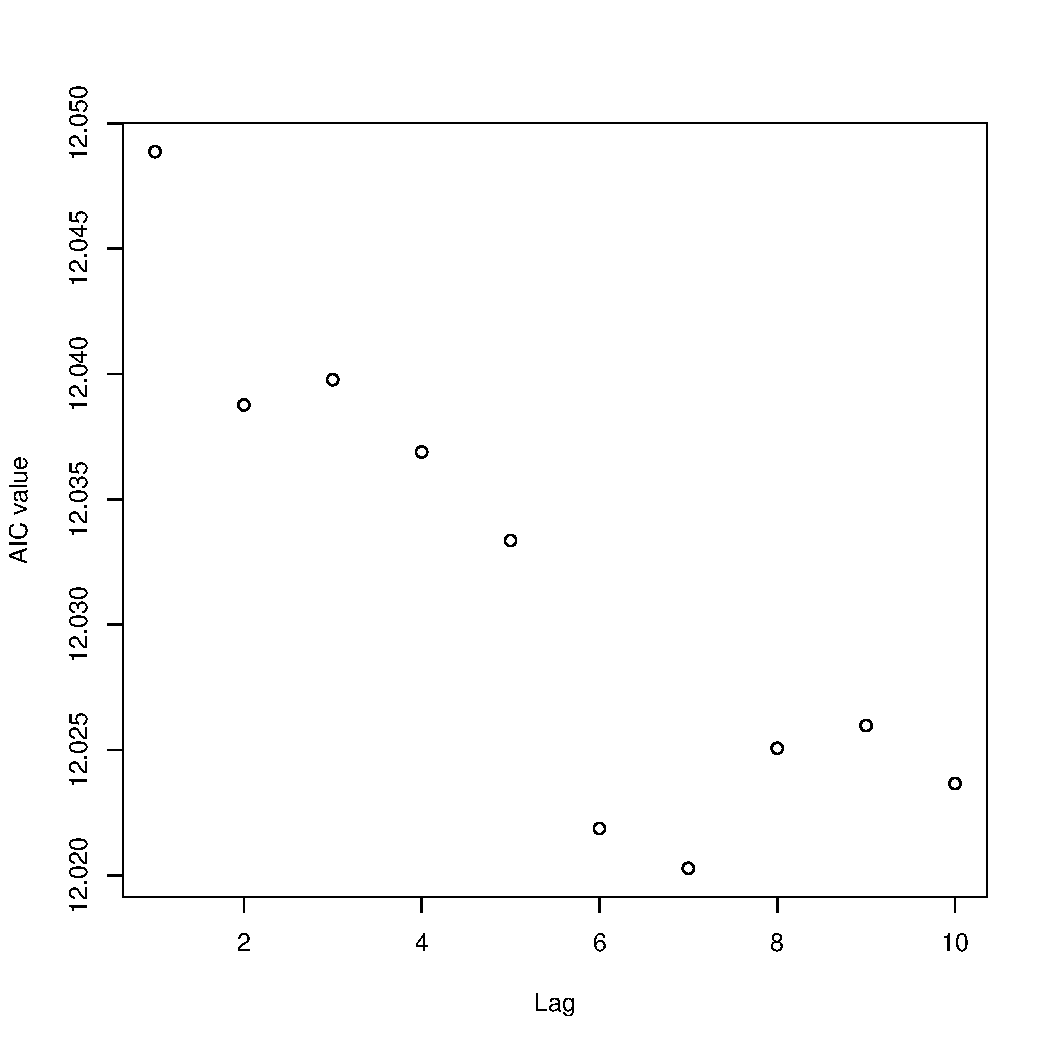
\includegraphics[width=.45\textwidth]{1.Projekt_kode/Billeder/AIC_Lag_for_SE.pdf}}\quad
  \subfloat[][Ripple \& Ethereum]{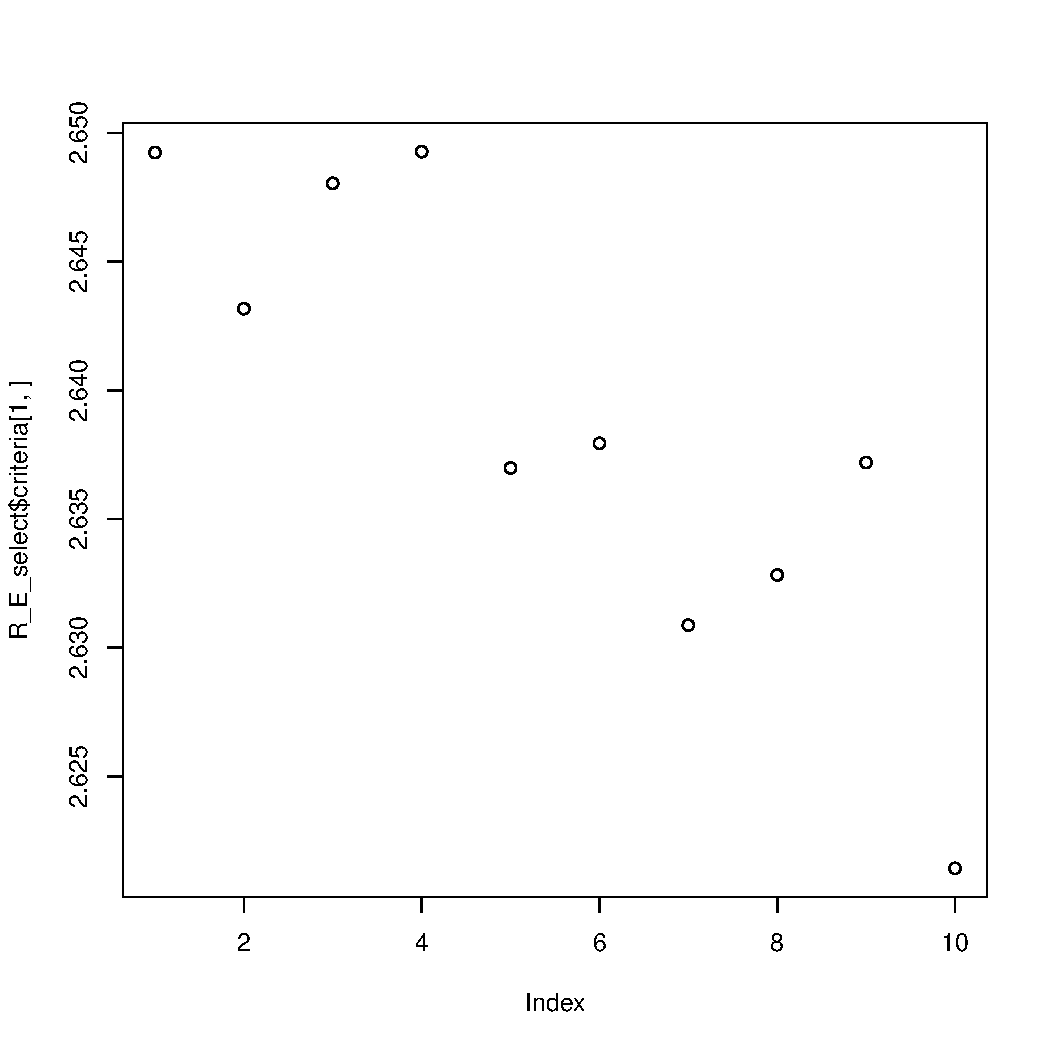
\includegraphics[width=.45\textwidth]{1.Projekt_kode/Billeder/AIC_Lag_for_RE.pdf}}\\
  \subfloat[][Ethereum \& Solana]{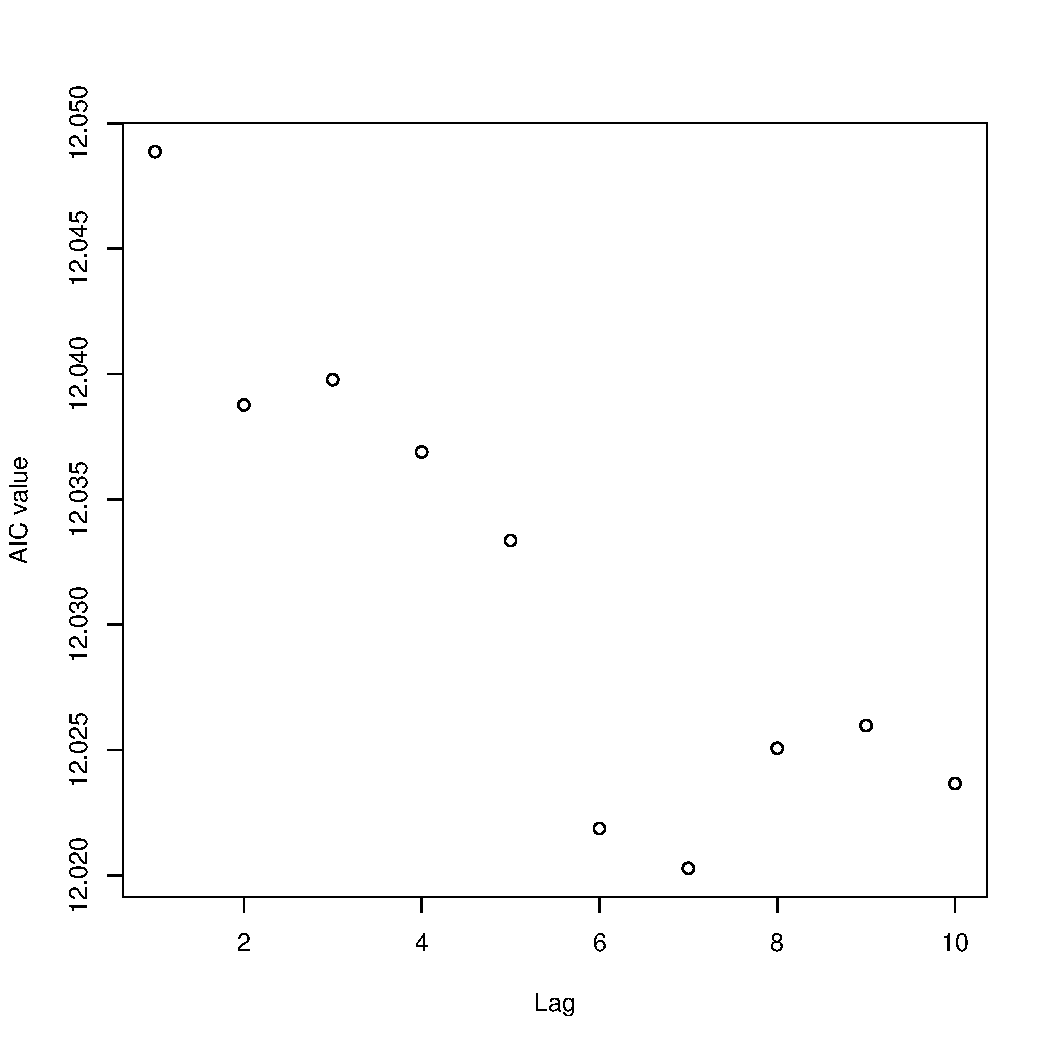
\includegraphics[width=.45\textwidth]{1.Projekt_kode/Billeder/AIC_Lag_for_ES.pdf}}\quad
  \subfloat[][Ripple \& Solana]{\includegraphics[width=.45\textwidth]{1.Projekt_kode/Billeder/AIC_Lag_for_RS.pdf}}
  \caption{AIC values for all combinations}
  \label{fig:AIC_plots}
\end{figure}
\noindent The lag order is chosen to be $VAR(6)$, $VAR(10)$, $VAR(6)$ and $VAR(6)$ respectively for each case. With the lag order determined. We can now build the VECM, where the lag order is simply one less than the $VAR$ counterpart.

\noindent The VECM is specified as follows, represented as a system of equations:\\

\begin{center}
    \textbf{SOL \& ETH}
\end{center}
$\text{Cointegrating Equation:} \quad  \beta = 1, \quad -0.03250492 \cdot \text{Ethereum} \\
\text{Equations:}$
\begin{align*} \quad
\Delta \text{Solana}_t &= 
\underset{(0.0039)}{-0.0073} \cdot \text{ECT}_{t-1} + 
\underset{(0.1414)}{0.0599} + 
\underset{(0.0346)}{0.0438} \cdot \Delta \text{Solana}_{t-1} \\
&\quad + \underset{(0.0016)}{-0.0026} \cdot \Delta \text{Ethereum}_{t-1} + 
\underset{(0.0348)}{-0.0151} \cdot \Delta \text{Solana}_{t-2} \\
&\quad + \underset{(0.0016)}{0.0017} \cdot \Delta \text{Ethereum}_{t-2} + 
\underset{(0.0349)}{0.0405} \cdot \Delta \text{Solana}_{t-3} \\
&\quad + \underset{(0.0016)}{0.0021} \cdot \Delta \text{Ethereum}_{t-3} + 
\underset{(0.0350)^{**}}{0.0962} \cdot \Delta \text{Solana}_{t-4} \\
&\quad + \underset{(0.0016)}{-0.0003} \cdot \Delta \text{Ethereum}_{t-4} + 
\underset{(0.0350)^{**}}{-0.0961} \cdot \Delta \text{Solana}_{t-5} \\
&\quad + \underset{(0.0016)}{-0.0009} \cdot \Delta \text{Ethereum}_{t-5} + \epsilon_{\text{Solana},t}
\end{align*}
\begin{align*}
 \quad
\Delta \text{Ethereum}_t &= 
\underset{(0.0828)}{-0.0516} \cdot \text{ECT}_{t-1} + 
\underset{(3.0230)}{2.2248} + 
\underset{(0.7403)^*}{-1.6153} \cdot \Delta \text{Solana}_{t-1} \\
&\quad + \underset{(0.0348)}{-0.0309} \cdot \Delta \text{Ethereum}_{t-1} + 
\underset{(0.7432)^*}{-1.6794} \cdot \Delta \text{Solana}_{t-2} \\
&\quad + \underset{(0.0348)}{0.0566} \cdot \Delta \text{Ethereum}_{t-2} + 
\underset{(0.7460)}{-0.8543} \cdot \Delta \text{Solana}_{t-3} \\
&\quad + \underset{(0.0350)^*}{0.0829} \cdot \Delta \text{Ethereum}_{t-3} + 
\underset{(0.7476)^*}{1.8980} \cdot \Delta \text{Solana}_{t-4} \\
&\quad + \underset{(0.0353)}{-0.0107} \cdot \Delta \text{Ethereum}_{t-4} + 
\underset{(0.7478)}{0.4330} \cdot \Delta \text{Solana}_{t-5} \\
&\quad + \underset{(0.0350)^*}{-0.0711} \cdot \Delta \text{Ethereum}_{t-5} + \epsilon_{\text{Ethereum},t}
\end{align*}

%
\begin{center}
    \textbf{XRP \& ETH}
\end{center}
$\text{Cointegrating Equation:} \quad  \beta = 1, \quad -0.000267678 \cdot \text{Ethereum} \\
\text{Equations:} $
\begin{align*}
 \quad
\Delta \text{Ripple}_t &= 
\underset{(0.0068)}{-0.0130} \cdot \text{ECT}_{t-1} + 
\underset{(0.0013)}{0.0002} + 
\underset{(0.0350)}{-0.0452} \cdot \Delta \text{Ripple}_{t-1} \\
&\quad + \underset{(1.5 \times 10^{-5})}{-2.1 \times 10^{-5}} \cdot \Delta \text{Ethereum}_{t-1} + 
\underset{(0.0351)}{-0.0009} \cdot \Delta \text{Ripple}_{t-2} \\
&\quad + \underset{(1.5 \times 10^{-5})}{5.2 \times 10^{-6}} \cdot \Delta \text{Ethereum}_{t-2} + 
\underset{(0.0350)}{0.0348} \cdot \Delta \text{Ripple}_{t-3} \\
&\quad + \underset{(1.5 \times 10^{-5})}{-1.1 \times 10^{-6}} \cdot \Delta \text{Ethereum}_{t-3} + 
\underset{(0.0352)}{0.0069} \cdot \Delta \text{Ripple}_{t-4} \\
&\quad + \underset{(1.5 \times 10^{-5})^{*}}{3.9 \times 10^{-5}} \cdot \Delta \text{Ethereum}_{t-4} + \epsilon_{\text{Ripple},t}
\end{align*}
\begin{align*}
\quad
\Delta \text{Ethereum}_t &= 
\underset{(15.7856)}{21.8381} \cdot \text{ECT}_{t-1} + 
\underset{(2.9293)}{1.9563} + 
\underset{(81.1699)^{**}}{-236.2089} \cdot \Delta \text{Ripple}_{t-1} \\
&\quad + \underset{(0.0349)}{-0.0100} \cdot \Delta \text{Ethereum}_{t-1} + 
\underset{(81.4008)}{-76.8518} \cdot \Delta \text{Ripple}_{t-2} \\
&\quad + \underset{(0.0348)}{0.0226} \cdot \Delta \text{Ethereum}_{t-2} + 
\underset{(81.3764)}{131.9577} \cdot \Delta \text{Ripple}_{t-3} \\
&\quad + \underset{(0.0348)}{0.0125} \cdot \Delta \text{Ethereum}_{t-3} + 
\underset{(81.6781)^{*}}{-207.0333} \cdot \Delta \text{Ripple}_{t-4} \\
&\quad + \underset{(0.0353)^{**}}{0.0918} \cdot \Delta \text{Ethereum}_{t-4} + \epsilon_{\text{Ethereum},t}
\end{align*}


%
\begin{center}
   \textbf{ETH \& SOL}
\end{center}
$\text{Cointegrating Equation:} \quad  \beta = 1, \quad -25.22835 \cdot \text{Solana} \\
\text{Equations:} $
\begin{align*}
 \quad
\Delta \text{Ethereum}_t &= 
\underset{(0.0037)}{0.0011} \cdot \text{ECT}_{t-1} + 
\underset{(3.7672)}{1.9951} + 
\underset{(0.0348)}{-0.0304} \cdot \Delta \text{Ethereum}_{t-1} \\
&\quad + \underset{(0.7403)^*}{-1.6282} \cdot \Delta \text{Solana}_{t-1} + 
\underset{(0.0349)}{0.0570} \cdot \Delta \text{Ethereum}_{t-2} \\
&\quad + \underset{(0.7434)^*}{-1.6930} \cdot \Delta \text{Solana}_{t-2} + 
\underset{(0.0350)^*}{0.0835} \cdot \Delta \text{Ethereum}_{t-3} \\
&\quad + \underset{(0.7462)}{-0.8698} \cdot \Delta \text{Solana}_{t-3} + 
\underset{(0.0353)}{-0.0101} \cdot \Delta \text{Ethereum}_{t-4} \\
&\quad + \underset{(0.7478)^*}{1.8819} \cdot \Delta \text{Solana}_{t-4} + 
\underset{(0.0350)^*}{-0.0703} \cdot \Delta \text{Ethereum}_{t-5} \\
&\quad + \underset{(0.7480)}{0.4150} \cdot \Delta \text{Solana}_{t-5} + \epsilon_{\text{Ethereum},t}
\end{align*}
\begin{align*}
 \quad
\Delta \text{Solana}_t &= 
\underset{(0.0002)^*}{0.0004} \cdot \text{ECT}_{t-1} + 
\underset{(0.1761)}{-0.1083} + 
\underset{(0.0016).}{-0.0027} \cdot \Delta \text{Ethereum}_{t-1} \\
&\quad + \underset{(0.0346)}{0.0443} \cdot \Delta \text{Solana}_{t-1} + 
\underset{(0.0016)}{0.0016} \cdot \Delta \text{Ethereum}_{t-2} \\
&\quad + \underset{(0.0348)}{-0.0146} \cdot \Delta \text{Solana}_{t-2} + 
\underset{(0.0016)}{0.0020} \cdot \Delta \text{Ethereum}_{t-3} \\
&\quad + \underset{(0.0349)}{0.0411} \cdot \Delta \text{Solana}_{t-3} + 
\underset{(0.0017)}{-0.0004} \cdot \Delta \text{Ethereum}_{t-4} \\
&\quad + \underset{(0.0350)^{**}}{0.0969} \cdot \Delta \text{Solana}_{t-4} + 
\underset{(0.0016)}{-0.0010} \cdot \Delta \text{Ethereum}_{t-5} \\
&\quad + \underset{(0.0350)^{**}}{-0.0954} \cdot \Delta \text{Solana}_{t-5} + \epsilon_{\text{Solana},t}
\end{align*}


%
\begin{center}
    \textbf{XRP \& SOL}
\end{center}
$\text{Cointegrating Equation:} \quad  \beta = 1, \quad -0.006285195 \cdot \text{Solana}\\
\text{Equations:} $
\begin{align*}
 \quad
\Delta \text{Ripple}_t &= 
\underset{(0.0039)}{-0.0015} \cdot \text{ECT}_{t-1} + 
\underset{(0.0015)}{0.0004} + 
\underset{(0.0301)^*}{-0.0661} \cdot \Delta \text{Ripple}_{t-1} \\
&\quad + \underset{(0.0003)}{-0.0003} \cdot \Delta \text{Solana}_{t-1} + 
\underset{(0.0302)}{0.0163} \cdot \Delta \text{Ripple}_{t-2} \\
&\quad + \underset{(0.0003)}{-0.0003} \cdot \Delta \text{Solana}_{t-2} + 
\underset{(0.0302)}{0.0307} \cdot \Delta \text{Ripple}_{t-3} \\
&\quad + \underset{(0.0003)}{-0.0001} \cdot \Delta \text{Solana}_{t-3} + 
\underset{(0.0302)}{0.0386} \cdot \Delta \text{Ripple}_{t-4} \\
&\quad + \underset{(0.0003)}{0.0003} \cdot \Delta \text{Solana}_{t-4} + 
\underset{(0.0301)}{-0.0262} \cdot \Delta \text{Ripple}_{t-5} \\
&\quad + \underset{(0.0003)}{-0.0002} \cdot \Delta \text{Solana}_{t-5} + \epsilon_{\text{Ripple},t}
\end{align*}
\begin{align*}
 \quad
\Delta \text{Solana}_t &= 
\underset{(0.4185)^*}{0.8644} \cdot \text{ECT}_{t-1} + 
\underset{(0.1643)}{-0.0566} + 
\underset{(3.2581).}{-5.4031} \cdot \Delta \text{Ripple}_{t-1} \\
&\quad + \underset{(0.0298)}{0.0270} \cdot \Delta \text{Solana}_{t-1} + 
\underset{(3.2626)}{2.7956} \cdot \Delta \text{Ripple}_{t-2} \\
&\quad + \underset{(0.0297)}{-0.0038} \cdot \Delta \text{Solana}_{t-2} + 
\underset{(3.2643)}{2.5712} \cdot \Delta \text{Ripple}_{t-3} \\
&\quad + \underset{(0.0297).}{0.0543} \cdot \Delta \text{Solana}_{t-3} + 
\underset{(3.2634)}{-3.1369} \cdot \Delta \text{Ripple}_{t-4} \\
&\quad + \underset{(0.0299)^{**}}{0.0975} \cdot \Delta \text{Solana}_{t-4} + 
\underset{(3.2541)}{2.7547} \cdot \Delta \text{Ripple}_{t-5} \\
&\quad + \underset{(0.0300)^{***}}{-0.1220} \cdot \Delta \text{Solana}_{t-5} + \epsilon_{\text{Solana},t}
\end{align*}







\section{Johansen Model Building}
One of the advantages using the Johansen test, is its ability to detect cointegration among multiple time series at a time. This means that we are not only able to look at pairwise integrated series. We will throughout this secction both be using the trace test statistic explained in Section \cite{Johansen_test} and the Maximal Eigenvalue test. \\\\
The overall difference between the two tests is that the Trace test tests has $H_0$ saying there are at max $r$ cointegration relations versus $H_1$ stating the presence of more than $r$ cointegrating relations and has the statistic described in Section \cite{Johansen_test} \eqref{eq:lrmax_coint_r} where the Maximal Eigenvalue test has $H_0$ stating the presence of $r$ cointegrating relations whereas $H_1$ indicates the presence of $r+1$ cointegrating relations and has the test statistic $-Tln(1-\lambda_{r_0+1})$ meaning it tests each eigenvalue's influence individually.\\
Generally there is little to no difference between the results achieved through the two tests. The Trace test although are more likely to dismiss $H_0$ even though it might be true hence having higher probability of type 1 errors. At the same time the Trace test is more efficient in finding cointegration relations when they do exist and is more advantageous when multiple cointegration relations exists. Since both tests are beneficial in different scenarios it is preferable to perform both to see whether the comply with each other, and if not, examine further why this could be the case \citep{johansentestdifferences}.\\\\
After using the AIC then in the two day ahead prediction six lags gives the lowest AIC score meaning a $VAR(6)$ is the most efficient model whereas in the "ikke twodayahead" it is in the most instances preferable to use a $VAR(6)$-$VAR(7)$ model according to the AIC.


\subsection{Trace test}\label{subsec:johansen_trace}
Using Johansens trace test with a 5\% critical value is compared to the corresponding critical values for $r=0,\;r\leq1,\;r\leq 2,\;r\leq3$.
The results are computed using the R function $ca.jo$ and the results are plotted below.
\begin{table}[h!]
\centering
\begin{tabular}{|c|c|c|}
\hline
\textbf{Cointegrating Relations} & \textbf{Test Statistic} & \textbf{5\% Critical Values} \\ \hline
$r \leq 3$ & 0.32  & 8.18  \\ \hline
$r \leq 2$ & 13.85 & 17.95 \\ \hline
$r \leq 1$ & 42.19 & 31.52 \\ \hline
$r = 0$    & 83.51 & 48.28 \\ \hline
\end{tabular}
\caption{5\% $ca.jo$ results for the Johansen Trace test}
\label{tab:traceresults}
\end{table}
In Table \ref{tab:traceresults} it is seen that since the test statistic for $r=0$ and $r\leq1$ are more extreme than the critical values and thereby these null hypotheses are rejected  this indicates the presence of two cointegrating relations since this has a test statistic of 13.85 which is less than the corresponding critical value 17.95 and hence failing to reject the null hypothesis indicating the presence of two cointegrating relations.

\subsection{Maximum Eigenvalue test}
The Maximum Eigenvalue test is also used in order to see whether the two tests comply with each other. Once again th R function $ca.jo$ is used to compute the results and can be seen in the table below where the setup is the same as above.
\begin{table}[h!]
\centering
\begin{tabular}{|c|c|c|}
\hline
\textbf{Cointegrating Relations} & \textbf{Test Statistic} & \textbf{5\% Critical Values} \\ \hline
$r \leq 3$ & 0.32  & 8.18  \\ \hline
$r \leq 2$ & 13.53 & 14.90 \\ \hline
$r \leq 1$ & 28.33 & 21.07 \\ \hline
$r = 0$    & 41.32 & 27.14 \\ \hline
\end{tabular}
\caption{5\% $ca.jo$ results for the Johansen Maximun Eigenvalue test}
\label{tab:maximal_eigenvalue}
\end{table}
Just as concluded in Section \ref{subsec:classification_of_various_hypot} then the Maximum Eigenvalue test also indicates two cointegrating relations and there are therefore no issues regarding contradictions in the tests.

\subsection{Model Choice}
After both the Trace test and the Maximum Eigenvalue test suggests the presence of two cointegrating relations the next step is to apply the achieved conclusions in forecasting. The R function $ca.jo$ indicates that of the four eigenvalues only the two greatest, 0.0324140, 0.0223421, are significant enough to indicate a cointegrating relations.\\
Next the R function $cajorls$ is used to fit a VECM with two cointegrating relations. The error correction terms, hence the two $\beta$ vectors are given as seen in the table below:\\
\begin{table}[h!]
\centering
\begin{tabular}{|c|c|c|}
\hline
\textbf{Cryptocurrency} & $\b{\beta}_1$ & $\b{\beta}_2$ \\ \hline
Bitcoin $t-7$  & $1.000000$  & $0.0000$      \\ \hline
Ethereum $t-7$  & $-5.684342 \cdot 10^{-14}$ & $1.0000$    \\\hline
Solana $t-7$  & $-2.218088 \cdot 10^3$ & $-22.5305$    \\ \hline
Ripple $t-7$  & $1.248777 \cdot 10^6$  & $6121.3729$   \\ \hline
\end{tabular}
\caption{ECT coefficients for selected assets.}
\label{tab:ect_coefficients}
\end{table}

\noindent Next the VECM will be transformed into a VAR model, using the R function \textit{vec2var}, which will be used to forecast in the following section.



\section{Forecast}
To evaluate models ability to correctly forecast, we first look at a plot of a single 20-day-ahead prediction. Secondly an 5-day-ahead forecast has been made iteratively, with each iteration adding another day to the training data set until the entire validation data set has been predicted upon. These predictions will be evaluated using the three different means mean absolute value (MAE), root mean square error(RMSE) and mean absolute percentage error(MAPE). The MAE is straight forward and measure the error value, while in the RMSE more weight is given to outliers. These two are a great combination, as a large difference between these two will indicate large outliers. The MAPE is used because it intuitively gives a great understanding of the errors. The formulas for calculation is given below:
\begin{align*}
    \text{MAE} = \frac{1}{n} \sum_{i=1}^{n} |y_i - \hat{y}_i|, \quad \text{RMSE} = \sqrt{\frac{1}{n} \sum_{i=1}^{n} (y_i - \hat{y}_i)^2}, \quad \text{MAPE} = \frac{1}{n} \sum_{i=1}^{n} \left| \frac{y_i - \hat{y}_i}{y_i} \right| \times 100.
\end{align*}
\noindent Where $y_i$ is the actual value and $\hat{y}_i$ is the predicted value and is the number of observation.

\subsection{Engel Granger}
First the 20-day-ahead predictions plot will looked at. These are however not very representable of the actual accuracy of the models, since it is just a single prediction. It does however give an insight if the model is able to capture the movements of the actual data.\\
\begin{center}
    \textbf{SOL \& ETH}
\end{center}
\begin{figure}[H]
  \centering
  \subfloat[][Solana]{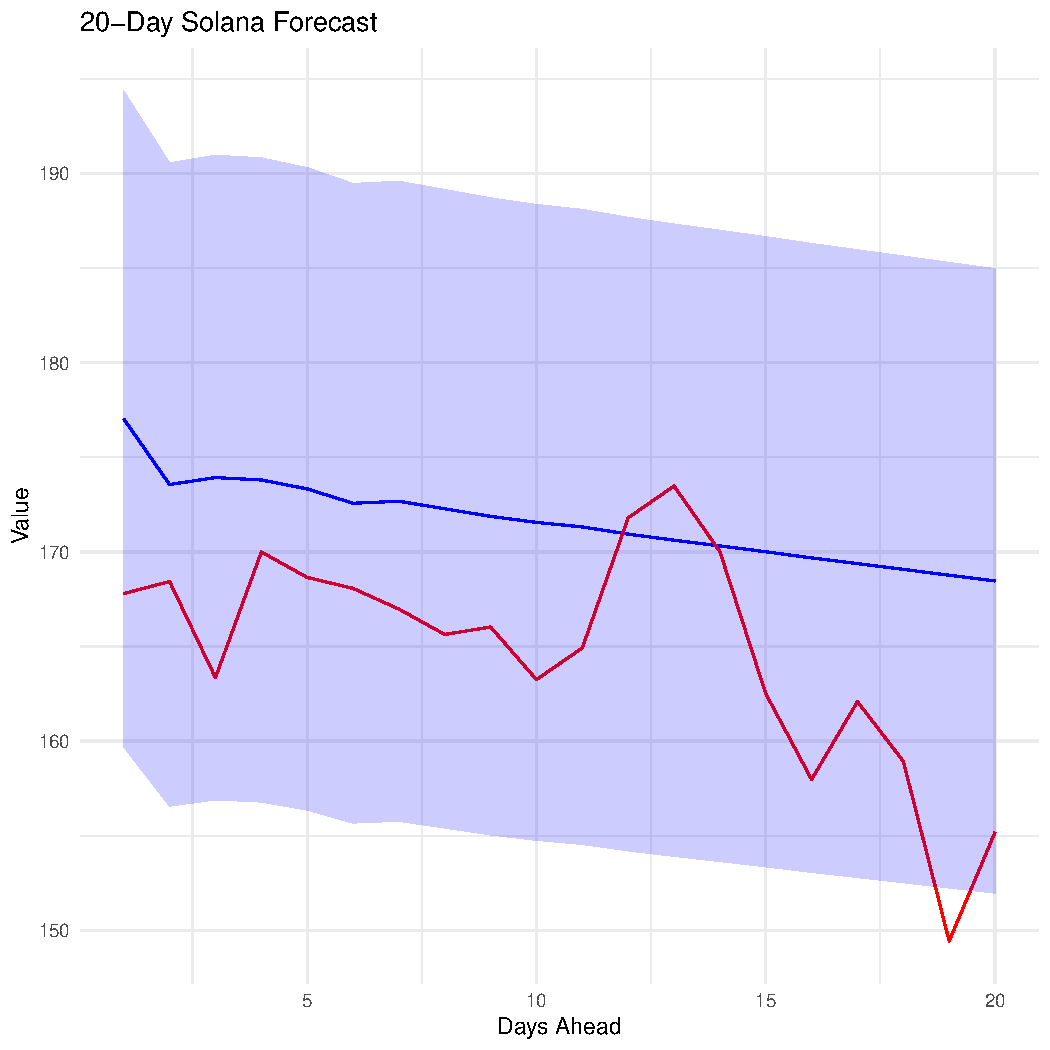
\includegraphics[width=.45\textwidth]{1.Projekt_kode/Billeder/20_day_ahead_plot_SolanaEthereum1.pdf}}\quad
  \subfloat[][Ethereum]{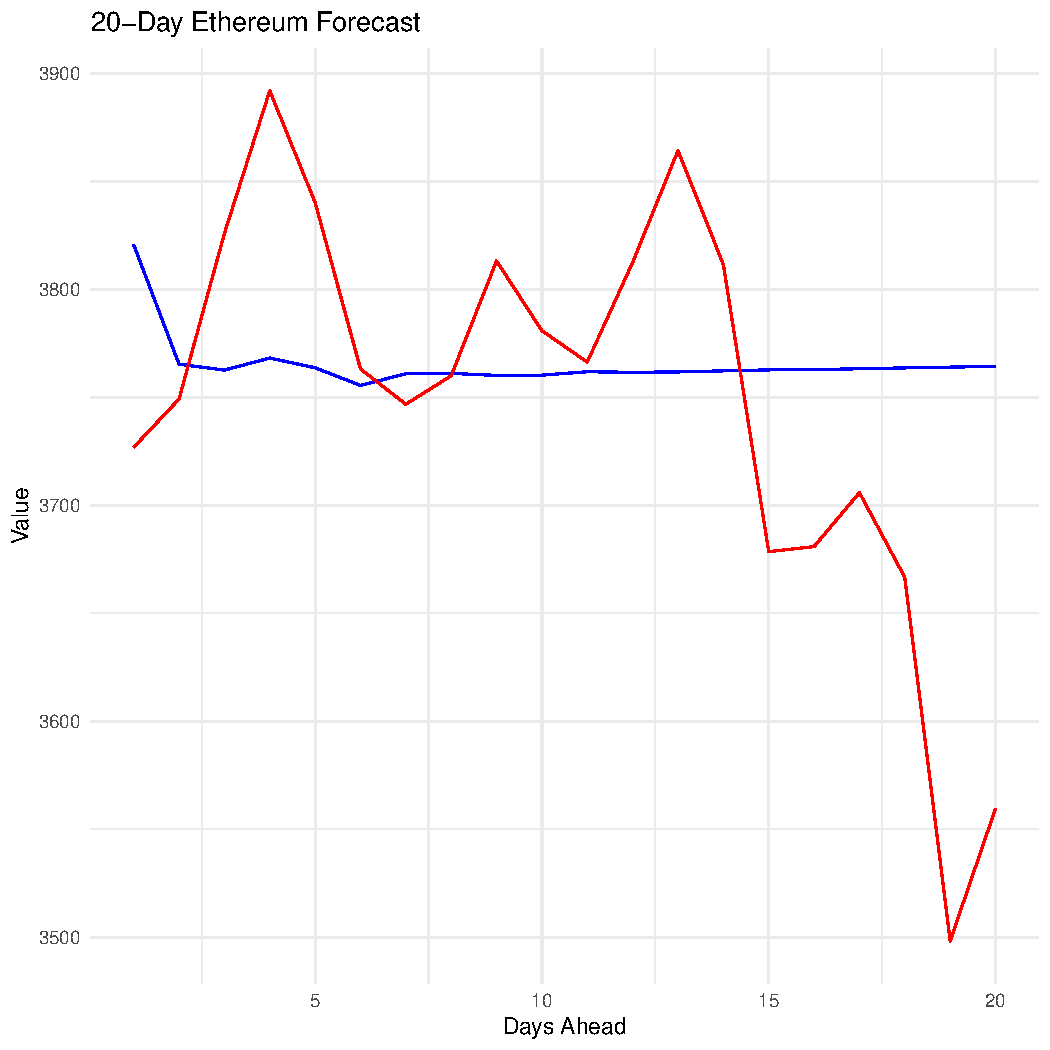
\includegraphics[width=.45\textwidth]{1.Projekt_kode/Billeder/20_day_ahead_plot_SolanaEthereum2.pdf}}
  \label{}
\end{figure}
\begin{center}
    \textbf{XRP \& ETH}
\end{center}
\begin{figure}[H]
  \centering
  \subfloat[][Ripple]{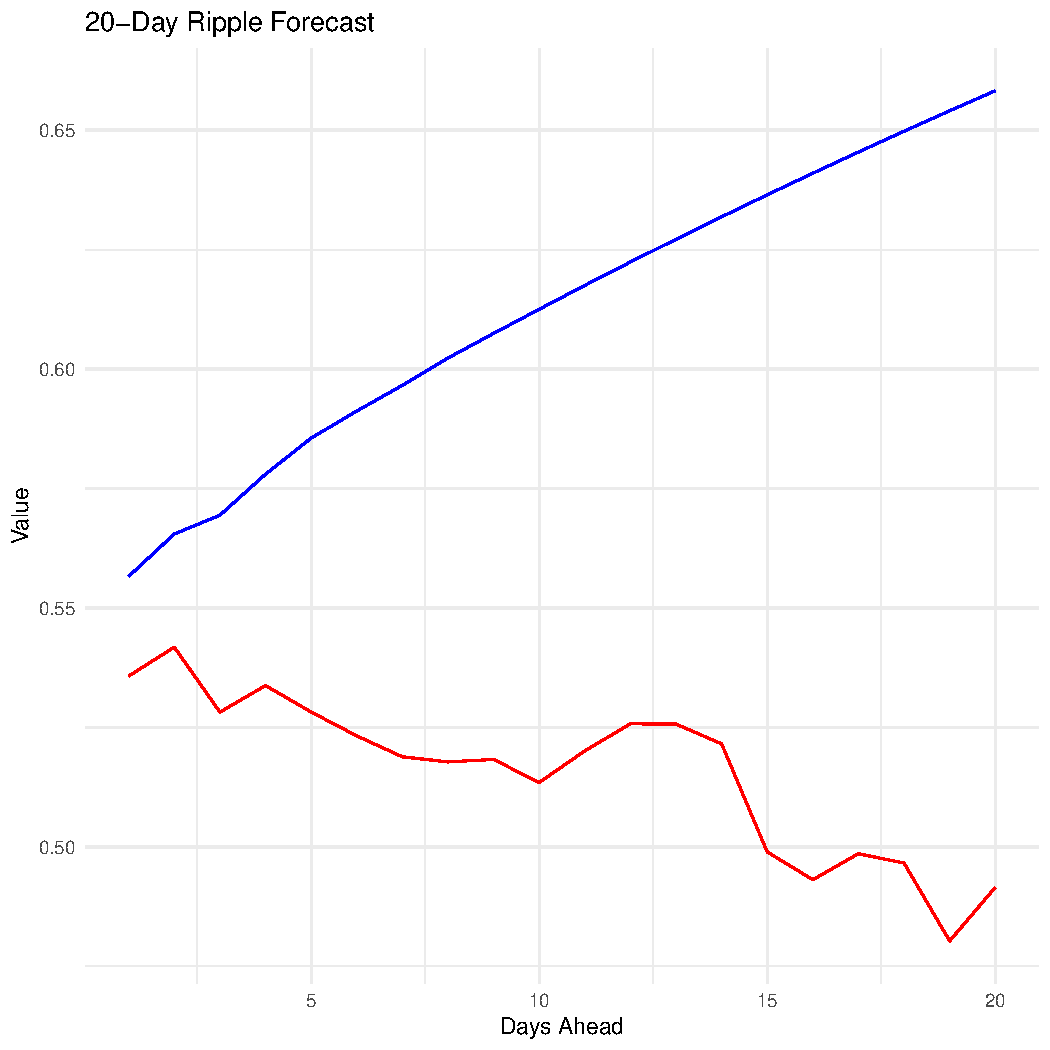
\includegraphics[width=.45\textwidth]{1.Projekt_kode/Billeder/20_day_ahead_plot_RippleEthereum1.pdf}}\quad
  \subfloat[][Ethereum]{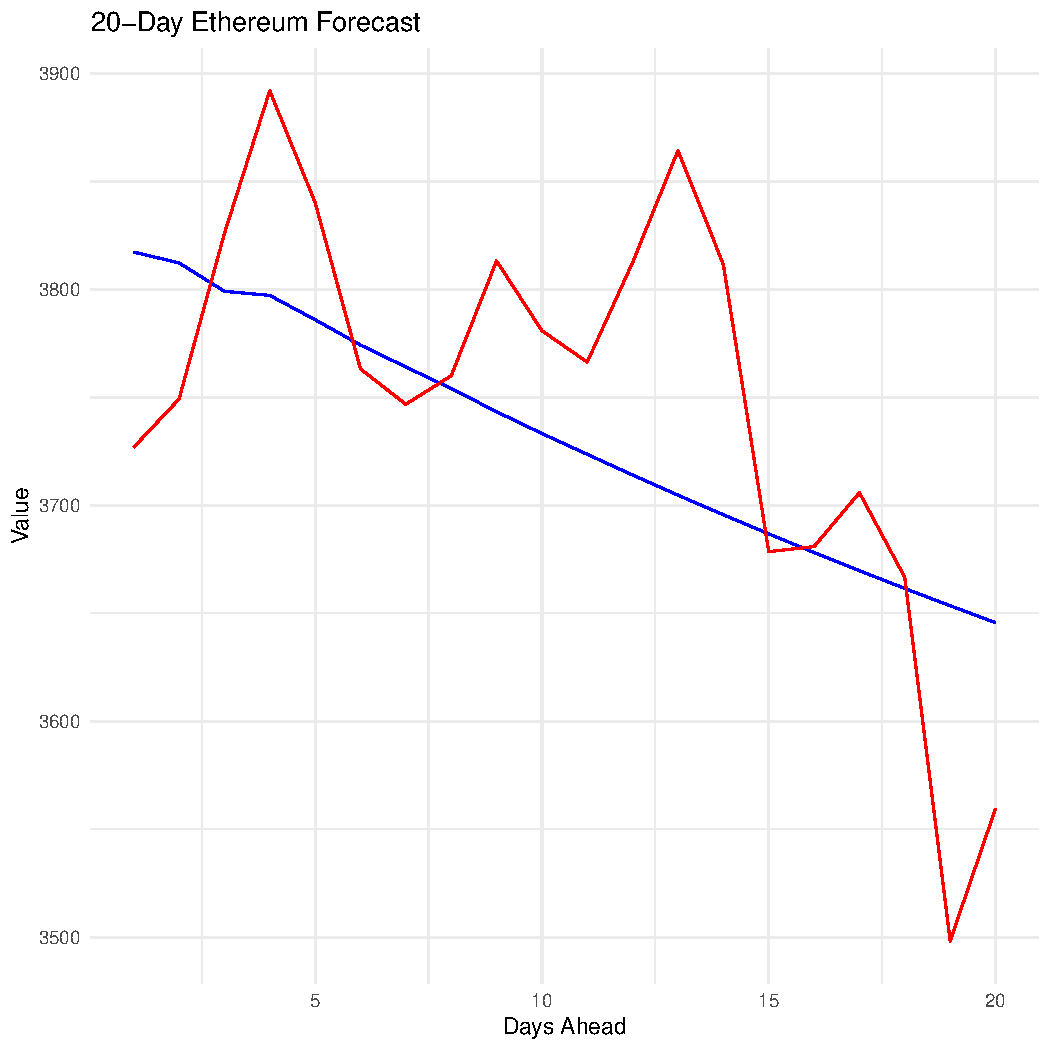
\includegraphics[width=.45\textwidth]{1.Projekt_kode/Billeder/20_day_ahead_plot_RippleEthereum2.pdf}}
  \label{}
\end{figure}
\begin{center}
    \textbf{ETH \& SOL}
\end{center}

\begin{figure}[H]
  \centering
  \subfloat[][Solana \& Ethereum]{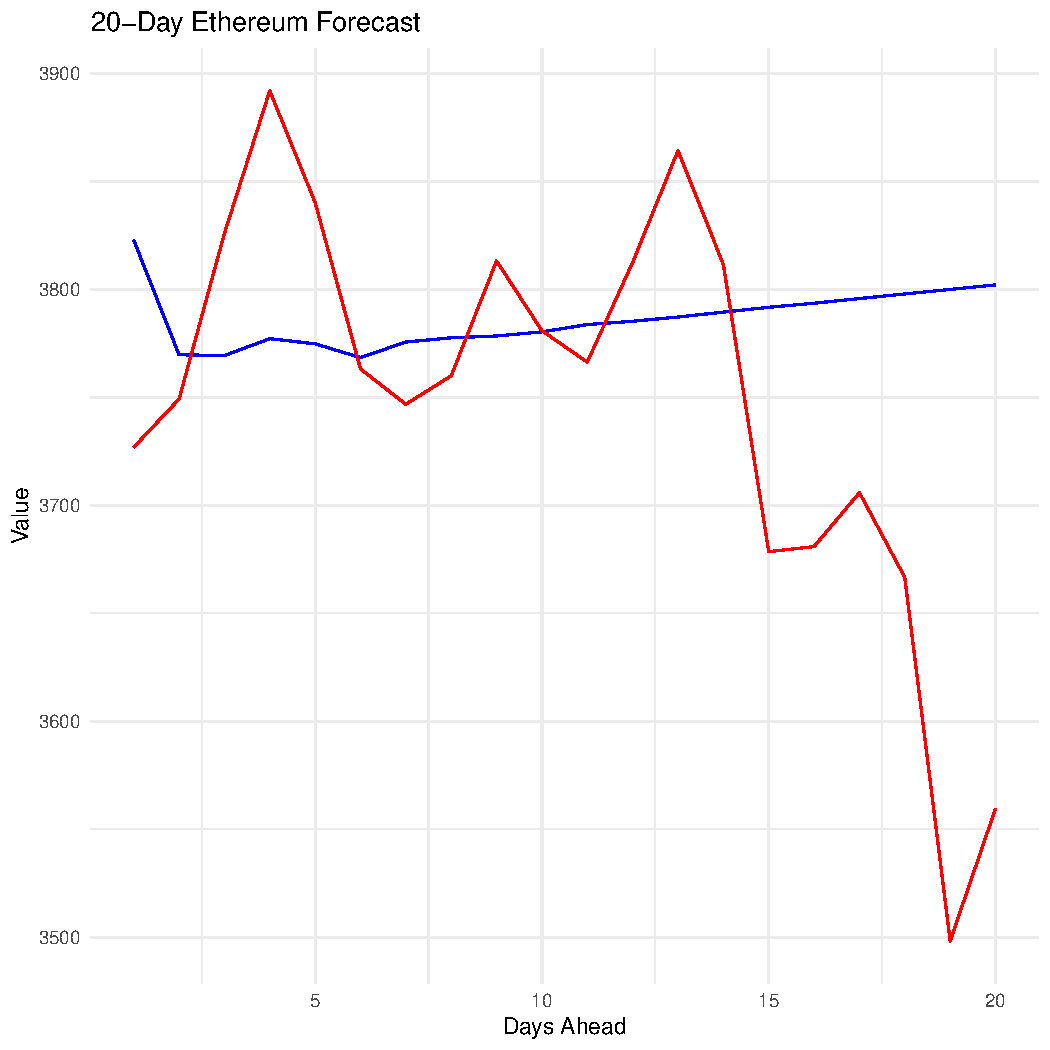
\includegraphics[width=.45\textwidth]{1.Projekt_kode/Billeder/20_day_ahead_plot_EthereumSolana1.pdf}}\quad
  \subfloat[][Ripple \& Ethereum]{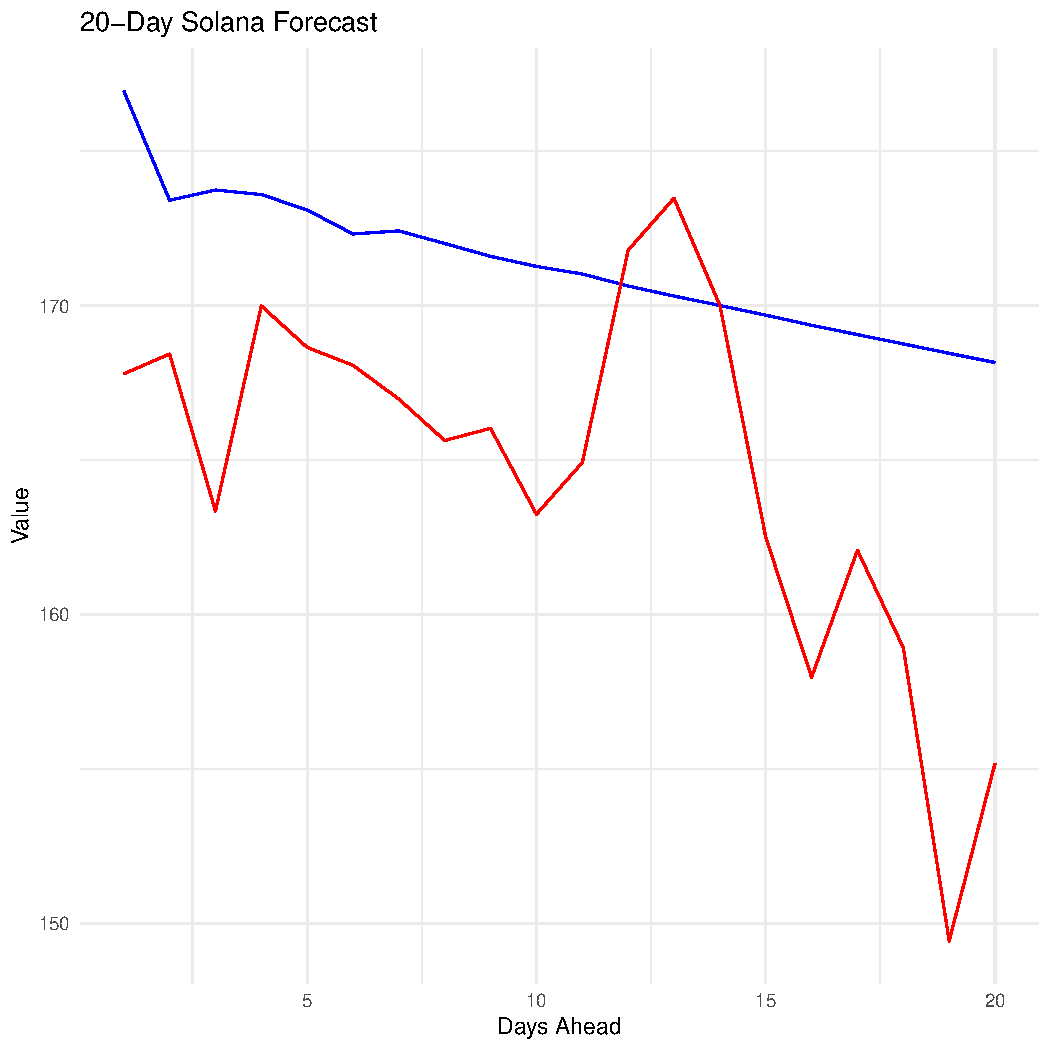
\includegraphics[width=.45\textwidth]{1.Projekt_kode/Billeder/20_day_ahead_plot_EthereumSolana2.pdf}}
  \label{}
\end{figure}
\begin{center}
    \textbf{XRP \& SOL}
\end{center}
\begin{figure}[H]
  \centering
  \subfloat[][Ripple]{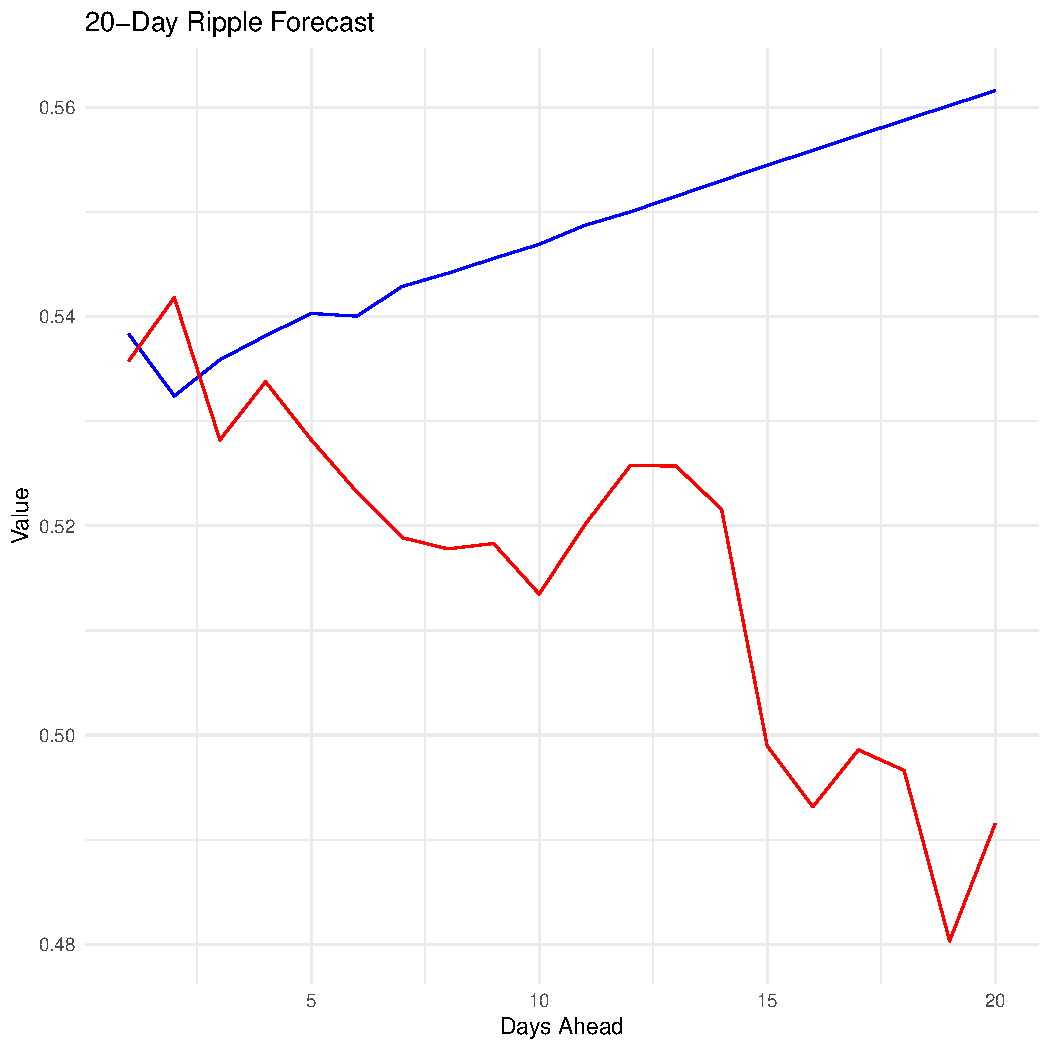
\includegraphics[width=.45\textwidth]{1.Projekt_kode/Billeder/20_day_ahead_plot_RippleSolana1.pdf}}\quad
  \subfloat[][Ethereum]{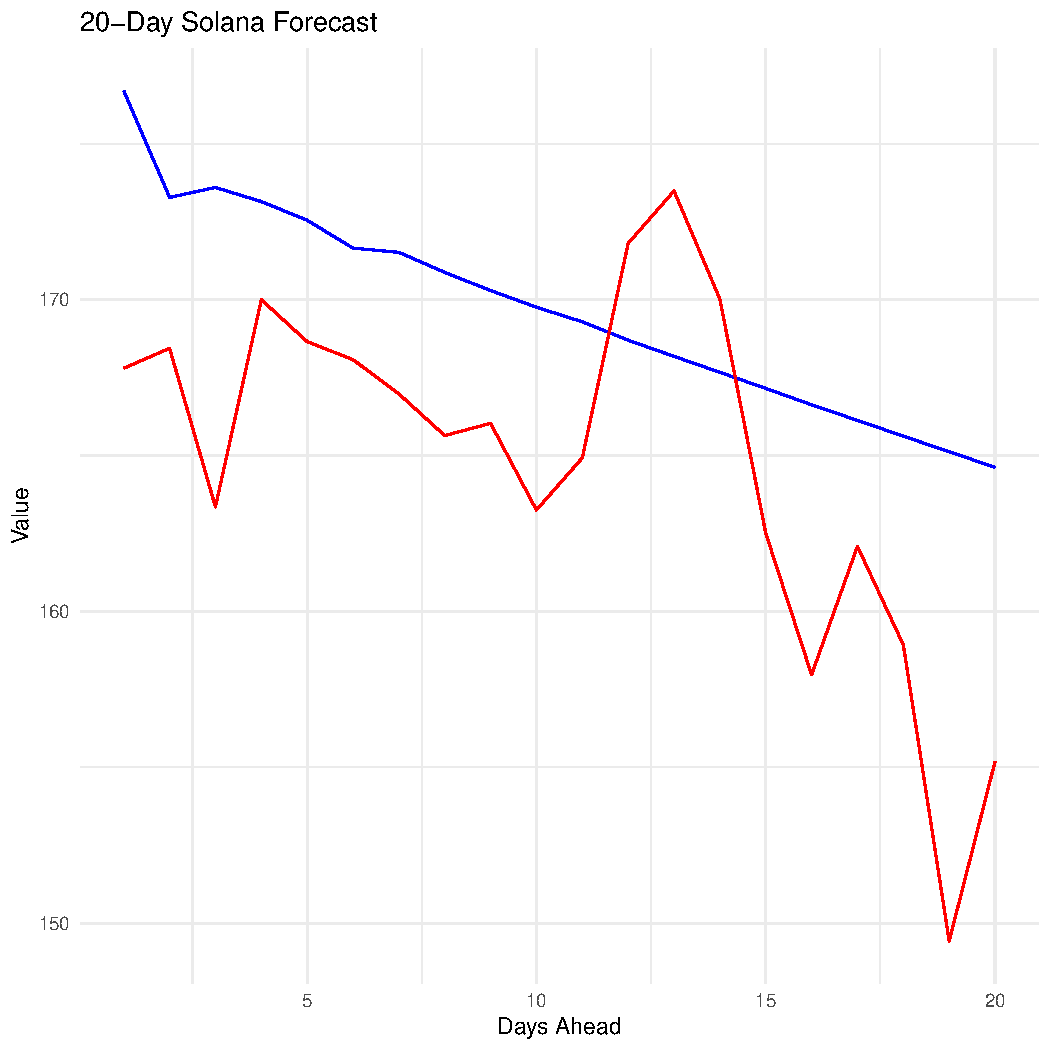
\includegraphics[width=.45\textwidth]{1.Projekt_kode/Billeder/20_day_ahead_plot_RippleSolana2.pdf}}
  \label{}
\end{figure}
\noindent For all the plots above it can be seen that the accuracy of the model do not seem to be high, which were to be expected, due to crypto currencies high volatility. Furthermore the models do not seem to capture the movement of the actual value. Some of the plots do capture the direction in which the currencies move, but without the nuances. It can be seen that the plots for the models of combination SOL \& ETH and ETH \& SOL looks identical which is to be expected since cointegration is not directionally. Below tables with the models level of predictability is stated:

\begin{table}[H]
\centering
\caption{Performance Metrics for Solana and Ethereum}
\begin{tabular}{lcccccc}
\toprule
\textbf{Metric} & \textbf{One-Day} & \textbf{Two-Day} & \textbf{Three-Day} & \textbf{Four-Day} & \textbf{Five-Day} \\
\midrule
\textbf{MAE} & & & & & \\
Solana        & 28.11133 & 25.22199 & 27.12728 & 27.9634 & 27.72747 \\
Ethereum      & 811.18274 & 771.61202 & 818.57316 & 845.9166 & 847.10831 \\
\midrule
\textbf{RMSE} & & & & & \\
Solana        & 31.24737 & 28.33555 & 30.14608 & 30.94042 & 30.63449 \\
Ethereum      & 953.08236 & 914.34242 & 956.88827 & 979.86588 & 979.72258 \\
\midrule
\textbf{MAPE} & & & & & \\
Solana        & 19.85790 & 17.85844 & 19.18544 & 19.77437 & 19.62114 \\
Ethereum      & 30.54404 & 29.21761 & 30.93889 & 31.95720 & 32.08274 \\
\bottomrule
\end{tabular}
\end{table}

\begin{table}[H]
\centering
\caption{Performance Metrics for Ripple and Ethereum}
\begin{tabular}{lcccccc}
\toprule
\textbf{Metric} & \textbf{One-Day} & \textbf{Two-Day} & \textbf{Three-Day} & \textbf{Four-Day} & \textbf{Five-Day} \\
\midrule
\textbf{MAE} & & & & & \\
Ripple        & 0.0448 & 0.0448 & 0.0473 & 0.0485 & 0.0503 \\
Ethereum      & 793.30 & 779.80 & 828.00 & 815.01 & 807.59 \\
\midrule
\textbf{RMSE} & & & & & \\
Ripple        & 0.0532 & 0.0523 & 0.0598 & 0.0617 & 0.0646 \\
Ethereum      & 936.56 & 922.12 & 965.61 & 951.38 & 943.21 \\
\midrule
\textbf{MAPE} & & & & & \\
Ripple        & 8.65 & 8.54 & 9.40 & 9.67 & 10.07 \\
Ethereum      & 29.92 & 29.51 & 31.27 & 30.87 & 30.69 \\
\bottomrule
\end{tabular}
\end{table}

\begin{table}[H]
\centering
\caption{Performance Metrics for Ethereum and Solana}
\begin{tabular}{lcccccc}
\toprule
\textbf{Metric} & \textbf{One-Day} & \textbf{Two-Day} & \textbf{Three-Day} & \textbf{Four-Day} & \textbf{Five-Day} \\
\midrule
\textbf{MAE} & & & & & \\
Ethereum      & 813.35 & 775.77 & 825.34 & 855.57 & 859.12 \\
Solana        & 28.06  & 25.11  & 26.96  & 27.77  & 27.52  \\
\midrule
\textbf{RMSE} & & & & & \\
Ethereum      & 955.04 & 918.29 & 963.20 & 988.58 & 990.43 \\
Solana        & 31.19  & 28.23  & 29.98  & 30.75  & 30.42  \\
\midrule
\textbf{MAPE} & & & & & \\
Ethereum      & 30.62  & 29.36  & 31.18  & 32.29  & 32.50  \\
Solana        & 19.82  & 17.78  & 19.07  & 19.64  & 19.47  \\
\bottomrule
\end{tabular}
\end{table}

\begin{table}[H]
\centering
\caption{Performance Metrics for Ripple and Solana}
\begin{tabular}{lcccccc}
\toprule
\textbf{Metric} & \textbf{One-Day} & \textbf{Two-Day} & \textbf{Three-Day} & \textbf{Four-Day} & \textbf{Five-Day} \\
\midrule
\textbf{MAE} & & & & & \\
Ripple        & 0.0451 & 0.0457 & 0.0453 & 0.0451 & 0.0450 \\
Solana        & 27.899 & 25.054 & 25.509 & 25.270 & 24.989 \\
\midrule
\textbf{RMSE} & & & & & \\
Ripple        & 0.0525 & 0.0533 & 0.0527 & 0.0525 & 0.0524 \\
Solana        & 31.035 & 28.167 & 28.550 & 28.267 & 27.901 \\
\midrule
\textbf{MAPE} & & & & & \\
Ripple        & 8.4753 & 8.5102 & 8.4825 & 8.4810 & 8.5048 \\
Solana        & 19.711 & 17.741 & 18.062 & 17.901 & 17.711 \\
\bottomrule
\end{tabular}
\end{table}
\noindent From the tables it stand out the prediction for Ripple in both the models in which it is represented. the two models are able to predict with an accuracy of less than $10\%$ in almost all cases. An interesting observation is that in som cases the MAPE is smaller for 5-day-ahead compared to the 1-day-ahead prediction. In the XRP \& SOL model, the MAE for Ripple remains somewhat constant for all five prediction. This is also the case for Ethereum's MAE in the XRP \& ETH model. It is left to conclude that the model XRP \& SOL is somewhat accurate and it is by for the one which makes the most accurate prediction for its respective crypto currencies.
\pause

\subsection{Johansen}
Like with Engel Granger forecast, we first inspect the 20-day-ahead prediction plots. 


\begin{table}[H]
\centering
\caption{Performance Metrics for Bitcoin, Ethereum, Solana, and Ripple}
\begin{tabular}{lccccc}
\toprule
\textbf{Metric} & \textbf{One-Day} & \textbf{Two-Day} & \textbf{Three-Day} & \textbf{Four-Day} & \textbf{Five-Day} \\
\midrule
\textbf{MAE} & & & & & \\
Bitcoin   & 436.5510 & 1360.4544 & 2096.0190 & 2372.9510 & 2839.9210 \\
Ethereum  &  29.4897 &   82.8389 &  112.3955 &  128.4171 &  154.1226 \\
Solana    &   5.3342 &    6.5635 &    8.9984 &   11.7554 &   10.2188 \\
Ripple    &   0.0118 &    0.0270 &    0.0461 &    0.0431 &    0.0531 \\
\midrule
\textbf{RMSE} & & & & & \\
Bitcoin   & 514.2976 & 1791.1630 & 2611.2730 & 2950.6350 & 3584.3680 \\
Ethereum  &  36.4638 &  106.7405 &  144.6352 &  162.4643 &  209.4623 \\
Solana    &   5.3489 &    8.0663 &   11.1579 &   14.3040 &   13.0975 \\
Ripple    &   0.0158 &    0.0317 &    0.0529 &    0.0506 &    0.0619 \\
\midrule
\textbf{MAPE} & & & & & \\
Bitcoin   &   0.7173 &    2.2203 &    3.4205 &    3.8782 &    4.6632 \\
Ethereum  &   0.9707 &    2.9081 &    3.9211 &    4.5413 &    5.5665 \\
Solana    &   3.6096 &    4.4267 &    6.0703 &    7.8966 &    6.8306 \\
Ripple    &   2.0972 &    5.1196 &    8.8016 &    8.0928 &   10.1982 \\
\bottomrule
\end{tabular}
\end{table}
\noindent In the table it can be seen that the MAE gets larger, the longer into the future we predict, this is to be expected, due to the high volatility of crypto currencies. The MAPE especially for ond-day-ahead is quint low across the board with bitcoin standing out as the best, with an prediction error of $0.72\%$ and reaching an error at five-day-ahead prediction of $4.66\%$. Just a single prediction namely five-day-ahead for Ripple is larger than $10\%$.\\
\textbf{forhold plot og table til hinanden.}